%%%%%%%%%%%%%%%%%%%%%%%%%%%%%%%%%%
% Felix Hoffmann, October 2014
% adapted from Jyotika Bahuguna October 2012
%%%%%%%%%%%%%%%%%%%%%%%%%%%%%%%%%%


%\documentclass{beamer}
\documentclass[xcolor=table,10pt]{beamer}
\usepackage{latexsym,amssymb,amsfonts,amsmath}
\usepackage{graphicx}
\usepackage{caption}
\usepackage{minted}
\usepackage{hyperref}
\usepackage{changepage} % for adjust width

%for Introduction - Part 1 - ... Orientation
%\useoutertheme[subsection=false, shadow]{miniframes} 
\useinnertheme{default}
\beamertemplatenavigationsymbolsempty

\usefonttheme{serif}
\usepackage{palatino}
\usepackage{eulervm} %additional math 


% Other Palatino font packages, with math
% see also http://tex.stackexchange.com/questions/89610
% and math_fonts.pdf in Latex docs
% --------------------
% \usepackage{pxfonts}
% \usepackage{mathpazo} % add possibly `sc` and `osf` options
% --------------------

\setbeamercolor*{structure}{fg=black}

\usepackage{transparent} % transparent graphics

\usepackage{textcomp}
\usepackage{subcaption}
\graphicspath{{img/}{../}}

\usepackage[table]{xcolor}
\usepackage{tikz}
\usetikzlibrary{arrows,shapes}
\usepackage{color}

%\usemintedstyle{friendly}
%\usemintedstyle{autumn}
%\usemintedstyle{manni}
%\usemintedstyle{tango}

\newminted[mlinepython]{python}{fontsize=\small, linenos,
               		numbersep=11pt,
               		gobble=4,
               		frame=lines,
                        bgcolor=bg,
               		framesep=3mm}    



% http://tex.stackexchange.com/questions/84936/
\usepackage[loadonly]{enumitem} % Enumitem-Beamer Incompatibility! See
                                % http://tex.stackexchange.com/a/52299/4912
\newlist{arrowlist}{itemize}{1}
\setlist[arrowlist]{label=$\Rightarrow$}


\usepackage[english]{babel}
\usepackage[latin1]{inputenc}

\usepackage{xcolor}

\usepackage[normalem]{ulem}
\hypersetup{%
  colorlinks=true,% hyperlinks will be coloured
  urlcolor=blue,
}
\makeatletter
\DeclareUrlCommand\ULurl@@{%
  \def\UrlFont{\ttfamily\color{blue}}%
  \def\UrlLeft{\uline\bgroup}%
  \def\UrlRight{\egroup}}
\def\ULurl@#1{\hyper@linkurl{\ULurl@@{#1}}{#1}}
\DeclareRobustCommand*\ULurl{\hyper@normalise\ULurl@}
\makeatother


\newenvironment{mydescription}[1]                                               
  {\begin{list}{}%
   {\renewcommand\makelabel[1]{\textbf{##1}\hfill}%
   \settowidth\labelwidth{\makelabel{#1}}%
   \setlength\leftmargin{\labelwidth}
   \addtolength\leftmargin{\labelsep}}}
  {\end{list}}

% cite source for content in the frame in bottom right corner
% usage: \source{here my source}
\usepackage[absolute,overlay]{textpos}
\setbeamercolor{framesource}{fg=gray}
\setbeamerfont{framesource}{size=\scriptsize}
\newcommand{\source}[1]{\begin{textblock*}{5cm}(7.7cm,8.9cm)
    \begin{beamercolorbox}[ht=0.5cm,right]{framesource}
        \usebeamerfont{framesource}\usebeamercolor[fg]{framesource} {#1}
    \end{beamercolorbox}
\end{textblock*}}

%%%%%%%%%%%%%%%%%%%%%%% stretching %%%%%%%%%%%%%%%%%%%%%%%%%%%%%%%

% from http://tex.stackexchange.com/questions/148365 
% and https://gist.github.com/navarroj/7789910

\let\svpar\par
\let\svitemize\itemize
\let\svenditemize\enditemize
\let\svitem\item
\def\newpar{\def\par{\svpar\vfill}}
\def\newitem{\def\item{\vfill\svitem}}
\let\svcenter\center
\let\svendcenter\endcenter
\let\svcolumn\column
\let\svendcolumn\endcolumn
\newlength\columnskip
\columnskip 0pt
\def\newcolumn{%
  \renewenvironment{column}[2]%
    {\svcolumn{##1}\setlength{\parskip}{\columnskip}##2}%
    {\svendcolumn\vspace{\columnskip}}}

\newcommand\stretchy{\only<2>{%
  \newpar\def\item{\svitem\newitem}%
  \renewenvironment{itemize}{\svitemize}{\svenditemize\newpar\par}%
  \renewenvironment{center}{\svcenter\newpar}{\svendcenter\newpar}%
  \newcolumn
}}

%%%%%%%%%%%%%%%%%%%%%%%%%%%%%%%%%%%%%%%%%%%%%%%%%%%%%%%%%%%%%%%%%%%%


\title {File operations, data parsing and batch files}
%\subtitle{}

\author[Felix Hoffmann]{Felix Hoffmann \vspace{0.25cm} \newline \small felix.hoffmann@jupiter.uni-freiburg.de} 
\institute[BCF]{Bernstein Center Freiburg}
\date{\today}


\AtBeginSection[]
{
\begin {frame}<beamer>
\frametitle{}
\tableofcontents[currentsection]
\end{frame}
}


%%%%%%%%%%%%%%%%%%%%%%%%%%%%%%%%%%%%%%%%%%%%%%

\begin{document}

\definecolor{bg}{rgb}{0.95,0.95,0.95}
\definecolor{tg}{rgb}{0.35,0.35,0.35}




\begin{frame} 
  \titlepage
\end{frame}



\begin{frame}{File operations and what ?}

  \begin{figure}
    \centering
    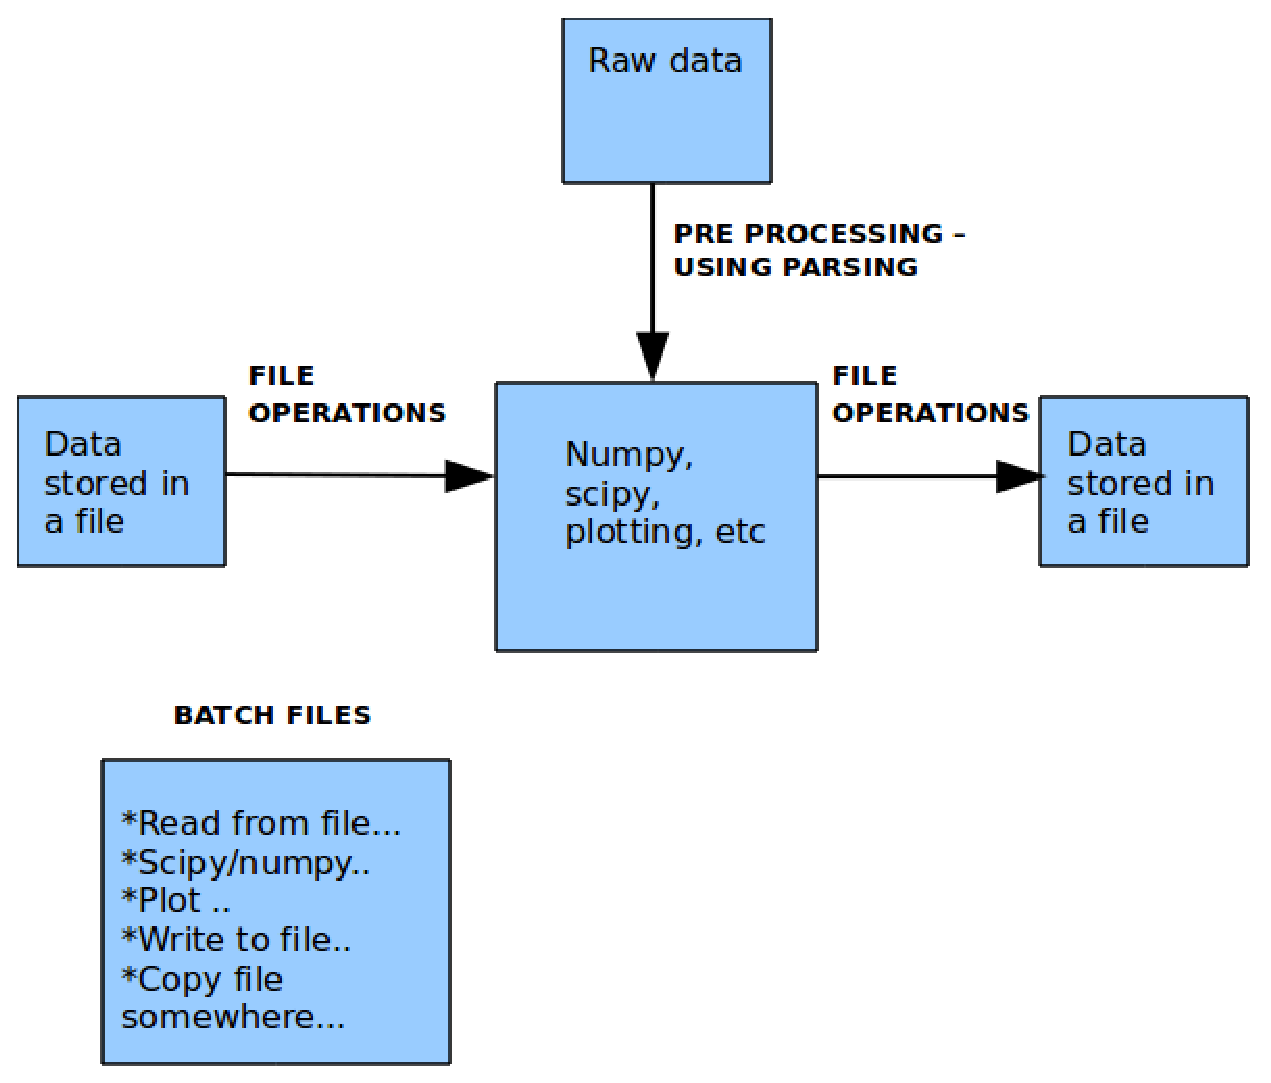
\includegraphics[width=3.0in]{Fits.eps}
  \end{figure}

\end{frame}



\section{Load/Save data}

\begin{frame}[fragile]{File operations: Reading}

  Opening an existing file 

  \begin{minted}{python}
    >>> f = open("test.txt","rb")
    >>> print f
    <open file 'test.txt', mode 'rb' at 0x...>
  \end{minted}
  \bigskip
  \pause
  Reading it:
  \begin{minted}{python}
    >>> f.read()
    'hello world'
  \end{minted}
  \pause
  \bigskip
  Closing it:
  \begin{minted}{python}
    >>> f.close()
    >>> print f
    <closed file 'test.txt', mode 'rb' at 0x...>
  \end{minted}

\end{frame}


\begin{frame}[fragile]

  \frametitle{File operations: Writing}

  Opening a (new) file 

  \begin{minted}{python}
    >>> f = open("new_test.txt","wb")
    >>> print f
    <open file 'test.txt', mode 'wb' at 0x...>
  \end{minted}
  \bigskip
  \pause
  Writing to it:
  \begin{minted}{python}
    >>> f.write("hello world, again")
    >>> f.write("... and again")
    >>> f.close()
  \end{minted}
  \pause
  \vspace{0.65cm}

  \begin{arrowlist}
  \item Only after calling close() the changes appear in the file for
    editing elsewhere!
  \end{arrowlist}

\end{frame}

\begin{frame}[fragile]{File operations: Appending}

  Opening an existing file 

  \begin{minted}{python}
    >>> f = open("test.txt","ab")
    >>> print f
    <open file 'test.txt', mode 'ab' at 0x...>
  \end{minted}
  \bigskip
  \pause  

  Appending to it:
  \begin{minted}{python}
    >>> f.write("hello world, again")
    >>> f.write("... and again")
    >>> f.close()
  \end{minted}
  \pause
  \vspace{0.8cm}

  \begin{arrowlist}
  \item In append mode the \textbf{file pointer} is set to the end of the opened file.
  \end{arrowlist}

\end{frame}


\begin{frame}[fragile]

  \frametitle{File operations: More about file pointers}

  \begin{mlinepython}
    f = open("lines_test.txt", "wb")
    for i in range(10):
        f.write("this is line %d \n" %(i+1))
    f.close()
  \end{mlinepython}
  \pause
  \bigskip

  Reading from the file:
  \smallskip

  \begin{minted}{python}
    >>> f = open("lines_test.txt", "rb")
    >>> f.readline()
  \end{minted}
  \pause
  \vspace{-10pt}
  \begin{minted}{python}
    'this is line 1 \n'
  \end{minted}
  \pause
  \vspace{-10pt}
  \begin{minted}{python}
    >>> f.readline()
  \end{minted}
  \pause
  \vspace{-10pt}
  \begin{minted}{python}
    'this is line 2 \n'
  \end{minted}
  \pause
  \vspace{-10pt}
  \begin{minted}{python}
    >>> f.read(14)
  \end{minted}
  \pause
  \vspace{-10pt}
  \begin{minted}{python}
    'this is line 3'
  \end{minted}
  \pause
  \vspace{-10pt}
  \begin{minted}{python}
    >>> f.read(2)
  \end{minted}
  \pause
  \vspace{-10pt}
  \begin{minted}{python}
    ' \n'
  \end{minted}

\end{frame}


\begin{frame}[fragile]
  \frametitle{File operations: More about file pointers}

  \begin{mydescription}{wbsssssssssssssssssssssssss}
    \itemsep4pt
    \item<1->[\texttt{f.tell()}] gives current position within file~\textbf{\texttt{f}}
    \item<2->[\texttt{f.seek(x[, from])}] change file pointer
      position within file~\textbf{\texttt{f}}, where 
      \hspace{0.2cm}\begin{mydescription}{wbssssssss}
        \itemsep0pt
        \item[\normalfont{from = 0}] from beginning of file
        \item[\normalfont{from = 1}] from current position
        \item[\normalfont{from = 2}] from end of file
      \end{mydescription}
  \end{mydescription}

  \bigskip
  \medskip
  \onslide<3->

  \begin{mlinepython}
    >>> f = open("lines_test.txt", "rb")
    >>> f.tell()
    0
    >>> f.read(10)
    'this is li'
    >>> f.tell()
    10
  \end{mlinepython}

\end{frame}


\begin{frame}[fragile]
  \frametitle{File operations: More about file pointers}
  \begin{mlinepython}
    >>> f.seek(5)
    >>> f.tell()
    5
    >>> f.seek(10,1)
    >>> f.tell()
    15
    >>> f.seek(-10,2)
    >>> f.tell()
    151
    >>> f.read()
    ' line 10 \n'
  \end{mlinepython}
\end{frame}

%

\begin{frame}[fragile]{File operations: Other Modes}
  %\stretchy

  \begin{mydescription}{wbssssssss}
    \itemsep22pt
    \item<1->[rb+] Opens a file for both reading and writing. The
      file pointer will be at the beginning of the file.
    \item<2->[wb+] Opens a file for both writing and
      reading. Overwrites the existing file if the file exists. If the file
      does not exist, creates a new file for reading and writing.
    \item<3->[ab+] Opens a file for both appending and reading in binary
      format. The file pointer is at the end of the file if the file
      exists. The file opens in the append mode. If the file does not exist,
      it creates a new file for reading and writing.
  \end{mydescription}

  \source{\url{tutorialspoint.com/python/python_files_io.htm}}
\end{frame}


\begin{frame}[fragile]
  \frametitle{Saving Data: Python Pickle}

  \onslide<1->
  Use pickle to save and retrieve more complex data types - lists,
  dictionaries and even class objects:

  \bigskip\pause

  \onslide<2>
  \begin{figure}
    \centering
    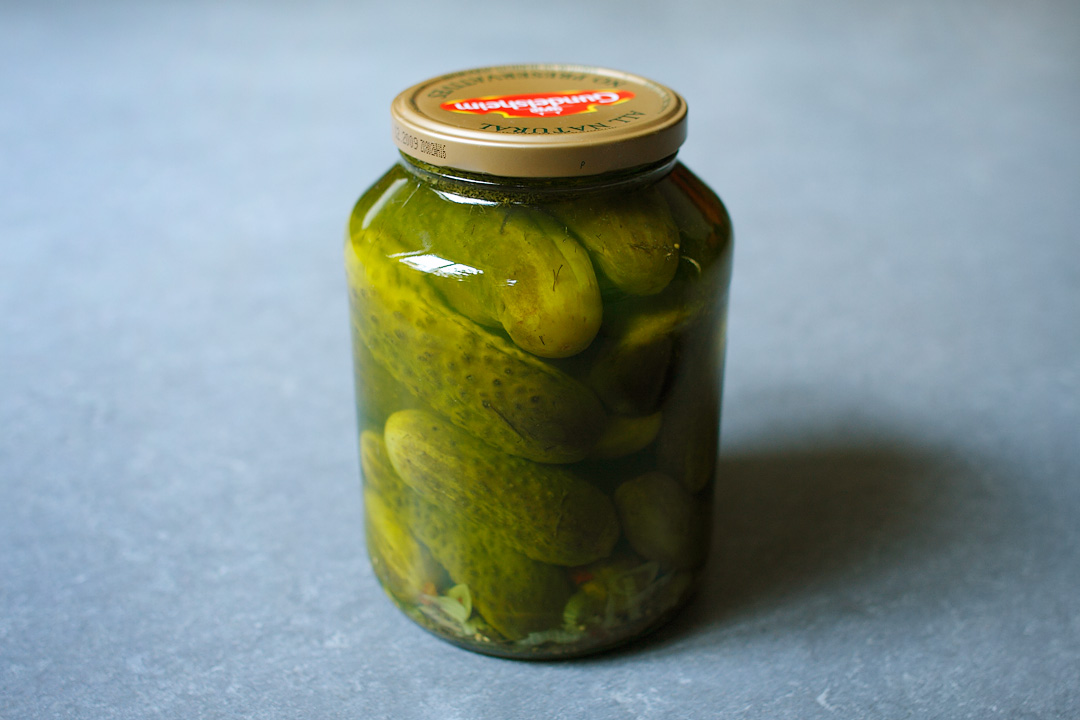
\includegraphics[width=6cm]{pickle.jpg}
    \caption*{\scriptsize  \textcopyright Dom Dada \href{http://creativecommons.org/licenses/by-nc-nd/2.0/}{CC BY-NC-ND 2.0}}
  \end{figure}
  
  \vspace{-5.6cm}
  \onslide<3->
  \begin{mlinepython}
    >>> import pickle 
    >>> f = open('save_file.p', 'wb')
    >>> ex_dict = {'hello': 'world'}
    >>> pickle.dump(ex_dict, f)
    >>> f.close()
  \end{mlinepython}

  \bigskip\onslide<4->

  \begin{mlinepython}
    >>> import pickle 
    >>> f = open('save_file.p', 'rb')
    >>> loadobj = pickle.load(f)
    >>> print loadobj['hello']
    world
  \end{mlinepython}

\end{frame}


\begin{frame}[fragile]
  \frametitle{Best practice: With Statement}


  \begin{mlinepython}
    import pickle 

    ex_dict = {'hello': 'world'}

    with open('save_file.p', 'wb') as f:
        pickle.dump(ex_dict, f)
  \end{mlinepython}

  \bigskip \pause
  \vspace{0.2cm}

  \begin{mlinepython}
    import pickle 

    with open('save_file.p', 'rb') as f:
        loadobj = pickle.load(f)

    print loadobj['hello']
  \end{mlinepython}
  \vspace{0.15cm}
  \begin{arrowlist}
  \item Use this!
  \end{arrowlist}

\end{frame}
















\section{Data parsing}

\begin{frame}{Need for parsing}
  % 
  \begin{columns}[T]
    %
    \begin{column}{.4\textwidth}
      Imagine that
      \vspace{0.5cm}
      \begin{arrowlist}
        \itemsep8pt
        \item[]<1-> Data files are generated by a third party (no control
          over the format)
        \item[]<2-> \& the data files need pre-processing
          \vspace{0.3cm}
        \item<3-> Regular expressions provide a powerful and concise way
          to perform pattern match/search/replace over the data
      \end{arrowlist}

    \end{column}
    %
    \begin{column}{.6\textwidth}
      \onslide<4->
      \begin{figure}
        
\includegraphics[width=6.4cm]{xkcd208.png}
        \caption*{\tiny  \textcopyright Randall Munroe \href{http://xkcd.com/208/}{xkcd.com} \href{http://creativecommons.org/licenses/by-nc/2.5/}{CC BY-NC 2.5}}
      \end{figure}
    \end{column}    

    %
  \end{columns}
  %
\end{frame}


\begin{frame}[fragile]
  \frametitle{Regular expressions - A case study}
  Formatting street names
  \vspace{0.4cm}
  \begin{minted}{python}
    >>> s = '100 NORTH MAIN ROAD'
  \end{minted}
  \pause
  \vspace{-10pt}
  \begin{minted}{python} 
    >>> s.replace('ROAD', 'RD.')
  \end{minted}
  \pause
  \vspace{-10pt}
  \begin{minted}{python} 
    '100 NORTH MAIN RD.'
  \end{minted}
  \pause
  \vspace{-10pt}
  \begin{minted}{python} 
    >>> s = '100 NORTH BROAD ROAD'
  \end{minted}
  \pause
  \vspace{-10pt}
  \begin{minted}{python}
    >>> s.replace('ROAD', 'RD.') 
  \end{minted}
  \pause
  \vspace{-10pt}
  \begin{minted}{python}
    '100 NORTH BRD. RD.'
  \end{minted}
  \pause
  \vspace{-10pt}
  \begin{minted}{python} 
    >>> s[:-4] + s[-4:].replace('ROAD', 'RD.') 
    '100 NORTH BROAD RD.'
  \end{minted}

  \vspace{0.3cm}
  Better use regular expressions!

  \begin{minted}{python}
    >>> import re 
    >>> re.sub(r'ROAD$', 'RD.', s) 
    '100 NORTH BROAD RD.'
  \end{minted}

  \source{example from Dive Into Python 3 \\ \textcopyright Mark Pilgrim 
    \href{http://creativecommons.org/licenses/by-sa/3.0/}{CC BY-SA 3.0}}

\end{frame}

\begin{frame}{Pattern matching with regular expressions}
\begin{adjustwidth}{2.5em}{0pt}
  \begin{mydescription}{wbbasdss}
    \itemsep3pt
    \item[\^]  Matches beginning of line/pattern
    \item[\$]  Matches end of line/pattern
    \item[. ]  Matches any character except newline
    \item[{[}..{]}]   Matches any single character in brackets
    \item[{[}\^..{]}]  Matches any single character not in brackets
    \item[re*]  Matches 0 or more occurrences of the preceding expression
    \item[re+]  Matches 1 or more occurrences of the preceding expression
    \item[re?]   Matches 0 or 1 occurrence
    \item[re\{n\}]  Match exactly n occurrences
    \item[re\{n,\}]   Match n or more occurrences
    \item[re\{n,m\}]   Match at least n and at most m
  \end{mydescription}
\end{adjustwidth}
  \vspace{0.3cm}
  \pause
  \begin{arrowlist}
    \item Use cheatsheets, trainers, tutorials, builders, etc..
  \end{arrowlist}
\end{frame}


\begin{frame}[fragile]{re.search() \& matches}

  \begin{minted}{python}
    >>> import re
    >>> data = "I like python"
    >>> m = re.search(r'python',data)
  \end{minted}
  \pause
  \vspace{-10pt}
  \begin{minted}{python}
    >>> print m
    <_sre.SRE_Match object at 0x...>
  \end{minted}
  \pause
  \vspace{0.7cm}
  Important properties of the match object:
  
  \begin{adjustwidth}{0.6cm}{0pt}
    \medskip
    \begin{mydescription}{wbasssss}
      \itemsep6pt
      \item[group()] Return the string matched by the RE
      \item[start()] Return the starting position of the match
      \item[end()] Return the ending position of the match
      \item[span()] Return a tuple containing the (start, end) positions of the match
    \end{mydescription}
  \end{adjustwidth}
  
\end{frame}


\begin{frame}[fragile]{re.search() \& matches}

  For example:

  \bigskip

  \begin{minted}{python}
    >>> import re
    >>> data = "I like python"
    >>> m = re.search(r'python',data)
  \end{minted}
  \pause
  \vspace{-10pt}
  \begin{minted}{python}
    >>> m.group()
    'python'
  \end{minted}
  \pause
  \vspace{-10pt}
  \begin{minted}{python}  
    >>> m.start()
    7
  \end{minted}
  \pause
  \vspace{-10pt}
  \begin{minted}{python} 
    >>> m.span()
    (7,13)
  \end{minted}

  \bigskip

  For a complete list of match object properties see for example the
  Python Documentation:

  \smallskip  

  \small \ULurl{https://docs.python.org/2/library/re.html#match-objects}

\end{frame}


\begin{frame}[fragile]{re.findall()}

  \begin{minted}{python}
    >>> import re
    >>> data = "Python is great. I like python"
    >>> m = re.search(r'[pP]ython',data)
  \end{minted}
  \pause
  \vspace{-10pt}
  \begin{minted}{python} 
    >>> m.group()
    'Python'
  \end{minted}

  \bigskip
  \pause
  \begin{arrowlist}
    \item  \textbf{re.search()} returns only the first match, use
      \textbf{re.findall()} instead:
  \end{arrowlist}
  \bigskip
  \pause

  \begin{minted}{python}
    >>> import re
    >>> data = "Python is great. I like python"
    >>> l = re.findall(r'[pP]ython',data)
  \end{minted}
  \pause
  \vspace{-10pt}
  \begin{minted}{python} 
    >>> print l
    ['Python', 'python']
  \end{minted}

  \bigskip
  \pause
  \begin{arrowlist}
    \item  Returns list instead of match object!
  \end{arrowlist}


\end{frame}


\begin{frame}[fragile]{re.findall() - Example}

  \begin{mlinepython}
    import re

    with open("history.txt", "rb") as f:
        text = f.read()

    year_dates = re.findall(r'19[0-9]{2}', text)
  \end{mlinepython}
 
\end{frame}

\begin{frame}[fragile]{re.split()}

  Suppose the data stream has well-defined delimiter

  \vspace{0.4cm}
  \begin{minted}{python}
    >>> data = "x = 20"
    >>> re.split(r'=',data)
    ['x ', ' 20']
  \end{minted}
  \vspace{0.2cm}
  \pause
  \begin{minted}{python} 
    >>> data = 'ftp://python.about.com'
    >>> re.split(r':/{1,3}', data)
    ['ftp', 'python.about.com']
  \end{minted}
  \vspace{0.2cm}
  \pause
  \begin{minted}{python}
    >>> data = '25.657'
    >>> re.split(r'\.',data)
    ['25', '657']
  \end{minted}


\end{frame}



\begin{frame}[fragile]{re.sub()}

  Replace patterns by other patterns.

  \medskip

  \begin{minted}{python}
    >>> data = "2004-959-559 # my phone number"
    >>> re.sub(r'#.*','',data)
    '2004-959-559 '
  \end{minted}
  \vspace{0.3cm}

  \pause
  A more interesting example:
  
  \medskip

  \begin{minted}{python}
    >>> data = "2004-959-559"
    >>> re.sub(r'([0-9]*)-([0-9]*)-([0-9]*)',
    >>>        r'\3-\2-\1', data)
  \end{minted}
  \pause
  \vspace{-10pt}
  \begin{minted}{python}             
    '559-959-2004'
  \end{minted}
  
  \vspace{0.3cm}
  \pause
  \begin{arrowlist}
    \item Groups are captured in parenthesis and referenced in the
      replacement string by \textbackslash1, \textbackslash2, ...
  \end{arrowlist}
\end{frame}



\section{Batch Files}

\begin{frame}[fragile]{os module}

  Provides a way of using os dependent functionality:

  \vspace{0.3cm}
  \begin{adjustwidth}{0.6cm}{0pt}
    \begin{mydescription}{wbbbaaaassss}
      \itemsep4pt
      \item[os.mkdir()]  Creates a directory (like mkdir)
      \item[os.chmod()]  Change the permissions (like chmod)
      \item[os.rename()]  Rename the old file name with the new file name.	
      \item[os.listdir()] List the contents of the directory
      \item[os.getcwd()] Get the current working directory path
      \item[os.path] Submodule for useful functions on pathnames
    \end{mydescription}
  \end{adjustwidth}

  \vspace{0.8cm}
  \pause
  For example, list all files in the current directory:

  \begin{minted}{python}
    >>> from os import listdir   
    >>>
    >>> for f in listdir("."):
    >>>     print f
  \end{minted}


\end{frame}




\end{document}

